% abtex2-modelo-artigo.tex, v-1.9.2 laurocesar
% Copyright 2012-2014 by abnTeX2 group at http://abntex2.googlecode.com/ 
%

% ------------------------------------------------------------------------
% ------------------------------------------------------------------------
% abnTeX2: Modelo de Artigo Acadêmico em conformidade com
% ABNT NBR 6022:2003: Informação e documentação - Artigo em publicação 
% periódica científica impressa - Apresentação
% ------------------------------------------------------------------------
% ------------------------------------------------------------------------

\documentclass[
	% -- opções da classe memoir --
	article,			% indica que é um artigo acadêmico
	11pt,				% tamanho da fonte
	oneside,			% para impressão apenas no verso. Oposto a twoside
	a4paper,			% tamanho do papel. 
	% -- opções da classe abntex2 --
	%chapter=TITLE,		% títulos de capítulos convertidos em letras maiúsculas
	%section=TITLE,		% títulos de seções convertidos em letras maiúsculas
	%subsection=TITLE,	% títulos de subseções convertidos em letras maiúsculas
	%subsubsection=TITLE % títulos de subsubseções convertidos em letras maiúsculas
	% -- opções do pacote babel --
	english,			% idioma adicional para hifenização
	brazil,				% o último idioma é o principal do documento
	sumario=tradicional
	]{abntex2}


% ---
% PACOTES
% ---

% ---
% Pacotes fundamentais 
% ---
\usepackage{lmodern}			% Usa a fonte Latin Modern
\usepackage[T1]{fontenc}		% Selecao de codigos de fonte.
\usepackage[utf8]{inputenc}		% Codificacao do documento (conversão automática dos acentos)
\usepackage{indentfirst}		% Indenta o primeiro parágrafo de cada seção.
\usepackage{nomencl} 			% Lista de simbolos
\usepackage{color}				% Controle das cores
\usepackage{graphicx}			% Inclusão de gráficos
\usepackage{microtype} 			% para melhorias de justificação
\usepackage{float}
% ---
		
% ---
% Pacotes adicionais, usados apenas no âmbito do Modelo Canônico do abnteX2
% ---
\usepackage{lipsum}				% para geração de dummy text
% ---
		
% ---
% Pacotes de citações
% ---
\usepackage[brazilian,hyperpageref]{backref}	 % Paginas com as citações na bibl
\usepackage[alf,num]{abntex2cite}	% Citações padrão ABNT
% ---

\usepackage{amsmath}

% ---
% Configurações do pacote backref
% Usado sem a opção hyperpageref de backref
\renewcommand{\backrefpagesname}{Citado na(s) página(s):~}
% Texto padrão antes do número das páginas
\renewcommand{\backref}{}
% Define os textos da citação
\renewcommand*{\backrefalt}[4]{
	\ifcase #1 %
		Nenhuma citação no texto.%
	\or
		Citado na página #2.%
	\else
		Citado #1 vezes nas páginas #2.%
	\fi}%
% ---

% ---
% Informações de dados para CAPA e FOLHA DE ROSTO
% ---
\titulo{Modelagem do Burnout em Ambientes Corporativos com Teoria dos Jogos e Algoritmos Genéticos}
\autor{Danilo Fonte}
\local{Brasil}
\data{Abril, 2025}
% ---

% ---
% Configurações de aparência do PDF final

% alterando o aspecto da cor azul
\definecolor{blue}{RGB}{41,5,195}

% informações do PDF
\makeatletter
\hypersetup{
     	%pagebackref=true,
		pdftitle={\@title}, 
		pdfauthor={\@author},
    	pdfsubject={Modelo de artigo científico com abnTeX2},
	    pdfcreator={LaTeX with abnTeX2},
		pdfkeywords={abnt}{latex}{abntex}{abntex2}{atigo científico}, 
		colorlinks=true,       		% false: boxed links; true: colored links
    	linkcolor=blue,          	% color of internal links
    	citecolor=blue,        		% color of links to bibliography
    	filecolor=magenta,      		% color of file links
		urlcolor=blue,
		bookmarksdepth=4
}
\makeatother
% --- 

% ---
% compila o indice
% ---
\makeindex
% ---

% ---
% Altera as margens padrões
% ---
\setlrmarginsandblock{3cm}{3cm}{*}
\setulmarginsandblock{3cm}{3cm}{*}
\checkandfixthelayout
% ---

% --- 
% Espaçamentos entre linhas e parágrafos 
% --- 

% O tamanho do parágrafo é dado por:
\setlength{\parindent}{1.3cm}

% Controle do espaçamento entre um parágrafo e outro:
\setlength{\parskip}{0.2cm}  % tente também \onelineskip

% Espaçamento simples
\SingleSpacing

% ----
% Início do documento
% ----
\begin{document}

% Retira espaço extra obsoleto entre as frases.
\frenchspacing 

\maketitle

\section*{Introdução}
\addcontentsline{toc}{section}{Introdução}

A síndrome de Burnout é um fenômeno associado à exaustão mental resultante de ambientes corporativos estressantes e exigentes. A Organização Mundial da Saúde (OMS) define o Burnout como um estado de estresse crônico relacionado ao trabalho, caracterizado por exaustão, cinismo e redução da eficácia profissional \cite{Downey2023}. Além disso, o acúmulo de expectativas não atendidas e o gerenciamento inadequado do estresse contribuem significativamente para o desenvolvimento dessa condição.

Em contextos corporativos modernos, o gerenciamento eficaz dos ciclos de estresse e recompensa dos funcionários é essencial para promover o bem-estar e o equilíbrio no ambiente de trabalho. A satisfação e a saúde mental dos colaboradores impactam diretamente a produtividade e a retenção de talentos, tornando-se fatores estratégicos para as organizações  \cite{Slusarz2022}.

Para lidar com essa questão, modelos baseados na Teoria dos Jogos Evolutivos oferecem uma abordagem promissora, pois permitem analisar como recompensas e penalidades impactam os trabalhadores ao longo do tempo. Esses modelos possibilitam encontrar um ponto de equilíbrio que maximize o engajamento e a satisfação dos conselheiros\cite{Sanfey2003}.

Neste contexto, este trabalho propõe o uso de Algoritmos Genéticos para otimizar o tabuleiro de um modelo previamente estabelecido por \cite{Zhang2020Burnout} de interação entre conselheiros e universidade. O objetivo é identificar um equilíbrio sustentável que maximize o bem-estar ao longo do tempo, considerando a dinâmica de recompensas e penalidades dentro da universidade \cite{Zhang2020Burnout}.

\section{Fundamentação Teórica}

\subsection{Definição do Burnout}
\begin{sloppypar}
\citeonline{freudenberger1974staff} foi o primeiro a propor o termo \textit{burnout}, definindo-o como um processo de exaustão mental e psicológica causado por demandas excessivas e irreais sobre os indivíduos. 
Desde então, diversos estudos têm caracterizado o burnout como ``uma síndrome de exaustão emocional, despersonalização e redução da realização pessoal, que ocorre com indivíduos que trabalham com pessoas de alguma forma'' \cite{maslach2001burnout, cordes1993review, benson2002burnout}. 
A Organização Mundial da Saúde (OMS) classifica o burnout como uma síndrome resultante de estresse crônico no ambiente de trabalho, caracterizada por exaustão, cinismo e redução da eficácia profissional \cite{Downey2023}.

As causas do burnout podem ser agrupadas em três categorias principais: fatores organizacionais e ambientais, fatores pessoais e características demográficas \cite{maslach2001burnout, benson2002burnout}. Entre os fatores organizacionais e ambientais, destacam-se o excesso de trabalho, os conflitos interpessoais e o ambiente organizacional. 
Nesse contexto, \citeonline{burke1996stress} identificam o excesso de trabalho como a principal causa do burnout.

Além dos aspectos organizacionais, fatores individuais também exercem influência significativa nesse processo. De acordo com \citeonline{cordes1993review, benson2002burnout}, profissionais idealistas, empáticos e com elevada sensibilidade emocional tendem a apresentar maior vulnerabilidade ao esgotamento.

Entre os principais efeitos do burnout estão a fadiga física, a exaustão mental, dificuldades para dormir e dores de cabeça. Além disso, podem surgir efeitos secundários, como problemas gastrointestinais e respiração acelerada, entre outros \cite{burke1996stress, freudenberger1974staff, benson2002burnout}.
\end{sloppypar}

\subsection{Descrição do Modelo Base}
O modelo utilizado como base para esta simulação foi proposto por \cite{Zhang2020Burnout} e descreve a interação entre orientador e a universidade. Para este estudo, esses agentes serão reinterpretados como funcionário e empresa, mantendo as mesmas características do modelo original. Assume-se que o funcionário seja um agente totalmente racional, capaz de identificar estratégias que maximizem seus ganhos e minimizem suas perdas, sempre considerando as recompensas ideais com base em expectativas presentes e futuras.

\subsubsection{Definição do custo de um Funcionário}

O custo de um funcionário pode ser analisado a partir de três componentes principais: custo atual, custo potencial e custo futuro.

\begin{itemize}
    \item O \textbf{custo atual} inclui fatores como tempo dedicado ao trabalho, carga de trabalho objetiva e o investimento em autoaperfeiçoamento.
    \item O \textbf{custo potencial} é determinado pelo desgaste mental e pelos custos relacionados à execução do trabalho, sendo influenciado negativamente por fatores externos, como burnout e eventos adversos.
    \item O \textbf{custo futuro} está associado à incerteza da carreira e às ações necessárias para o planejamento profissional do funcionário.
\end{itemize}

A equação que representa o custo total do funcionário é dada por:

\begin{equation}
    G = \beta_1 g_1 + \beta_2 g_2 + \beta_3 g_3
\end{equation}

\begin{equation}
    G = \beta_1 (s t + z - l) + \beta_2 (h^2 + c) + \beta_3 h^2
\end{equation}

Sujeito às seguintes condições:

\begin{equation}
    \beta_1, \beta_2, \beta_3 > 0, \quad \beta_1 + \beta_2 + \beta_3 = 1
\end{equation}

\begin{equation}
    0 < s, t, z, l, h, c < 1, \quad l < z
\end{equation}

Onde:

\begin{itemize}
    \item \( G \) representa o custo total do funcionário.
    \item \( g_1, g_2, g_3 \) correspondem, respectivamente, ao custo atual, custo potencial e custo futuro.
    \item \( s \) é o custo associado ao tempo dedicado ao trabalho.
    \item \( t \) representa a carga de trabalho objetiva.
    \item \( z \) é o custo de autoaperfeiçoamento.
    \item \( l \) mede a percepção do funcionário sobre a importância do autoaperfeiçoamento.
    \item \( h^2 \) refere-se ao custo do planejamento de carreira.
    \item \( c \) representa a possibilidade de eventos inesperados no ambiente de trabalho.
    \item Os coeficientes \( \beta_1, \beta_2, \beta_3 \) indicam a importância relativa de cada um dos custos, garantindo que sua soma seja igual a 1 (\( \beta_1 + \beta_2 + \beta_3 = 1 \)).
\end{itemize}

O modelo base também impõe restrições às variáveis, garantindo que:

\[
0 < s, t, z, l, h, c < 1, \quad l < z
\]

Isso reflete a premissa de que conselheiros mais consistentes em seu desempenho e planejamento de carreira tendem a apresentar um custo total reduzido e maior eficiência no trabalho.

\subsubsection{Definição do ganho de um funcionário}
O ganho de um funcionário é modelado a partir de três componentes: ganhos atuais (\( f_1 \)), ganhos potenciais (\( f_2 \)) e ganhos futuros (\( f_3 \)).

\begin{itemize}
    \item \textbf{Ganhos atuais}: incluem salário (\( d \)) e status profissional externo (\( e \)).
    \item \textbf{Ganhos potenciais}: referem-se ao planejamento de carreira (\( h_1 \)), autoaperfeiçoamento (\( l \)) e avaliação de performance (\( j \)), ponderada por \( \lambda_1 \).
    \item \textbf{Ganhos futuros}: abrangem o crescimento do funcionário na empresa, considerando carga de trabalho (\( st \)), planejamento de carreira e reconhecimento profissional.
\end{itemize}

O ganho total do funcionário (\( F \)) é expresso como:

\begin{equation}
    F = \alpha_1 f_1 + \alpha_2 f_2 + \alpha_3 f_3 = \alpha_1 (2d + e) + \alpha_2 (h_1 + l + \lambda_1 j) + \alpha_3 (st + h_1 + l + j)
\end{equation}

Onde:

\begin{equation}
    \alpha_1, \alpha_2, \alpha_3 > 0, \quad \alpha_1 + \alpha_2 + \alpha_3 = 1, \quad 0 < d, e, t, h_1, l, j, s < 1
\end{equation}

As perdas e ganhos líquidos (\( M \)) são dados por:

\begin{equation}
    M = F - G = 2\alpha_1 d + \alpha_2 e + (\alpha_2 + \alpha_3) h_1 - (\beta_2 + \beta_3) h_2 + (\alpha_2 + \alpha_3 + \beta_1) l 
\end{equation}

\begin{equation}
    + (\alpha_2 \lambda_1 + \alpha_3) j + (\alpha_3 - \beta_1) st - \beta_1 z - \beta_2 c
\end{equation}

Onde \( G \) representa os custos do funcionário, considerando planejamento de carreira (\( h_2 \)), autoaperfeiçoamento (\( z \)) e eventos inesperados (\( c \)).

O modelo sugere que um alto nível de autoaperfeiçoamento, planejamento de carreira e reconhecimento profissional resulta em maior ganho e menor custo para o funcionário.


\subsection{Teoria dos Jogos}

A teoria matemática dos jogos fornece uma base racional para a análise de uma ampla variedade de ações, setores e contextos do mundo real, especialmente aqueles fundamentados em interações competitivas que resultam em ganhos ou perdas para as partes envolvidas. Segundo \cite{morris1994introduction}, a teoria dos jogos possui dois objetivos principais: o primeiro é compreender por que os jogadores se comportam de determinada maneira em situações competitivas; o segundo é identificar quais são as melhores escolhas de ações ou jogadas para cada tipo de jogo ou situação.

De certo modo, pode-se dizer que cada um desses objetivos tem maior aplicabilidade em diferentes contextos, que podem ser agrupados em cenários de macro e micro escala. A macroescala refere-se a situações compostas por múltiplos jogadores, regras complexas e diversificadas, e com amplo impacto. Já a microescala diz respeito às estratégias e ações específicas que cada jogador deve adotar para maximizar seus ganhos ou minimizar perdas — especialmente em contextos onde essas perdas são inevitáveis \cite{morris1994introduction}.

\subsection{Equilibrio de Nash}

Considerando cenários cada vez mais dinâmicos e competitivos, a busca por minimizar perdas ou alcançar um ponto de equilíbrio entre os diversos jogadores ou agentes de um determinado sistema torna-se essencial. Segundo \citeonline{nash1951noncooperative}, todo jogo não cooperativo com um número finito de ações possui, ao menos em teoria, um ponto de equilíbrio que pode ser atingido em algum momento.

Esse ponto, conhecido como equilíbrio de Nash, ocorre quando um jogador não tem incentivo para alterar sua estratégia unilateralmente, desde que as estratégias dos demais permaneçam inalteradas. Em jogos finitos, portanto, cada participante tende a adotar uma estratégia de equilíbrio em relação aos demais \cite{nash1951noncooperative}.

\subsection{Problema das N-Rainhas}
O problema das N-Rainhas consiste em determinar o número total de configurações distintas \( Q(n) \) em que \( N \) rainhas podem ser posicionadas em um tabuleiro \( N \times N \) de forma que nenhuma delas se ataque mutuamente, ou seja, garantindo que não compartilhem a mesma linha, coluna ou diagonal. Esse problema é uma generalização do problema original das 8 rainhas, proposto por Max Bezzel em 1848 \cite{glock2022nqueens}. Em 1850, Franz Nauck \citeonline{nauck1850mathematik} encontrou uma solução para o problema das 8 rainhas e estendeu a formulação para o caso geral das \( N \) rainhas.

Estabelecendo uma correlação entre o problema das \( N \) rainhas e a Teoria dos Jogos, é possível tratá-lo como um jogo competitivo, no qual cada rainha busca minimizar a quantidade de ataques recebidos das demais. O ponto de equilíbrio é alcançado quando todas as rainhas estão posicionadas de forma que nenhuma possa atacar outra.

\subsection{Algoritmos Genéticos}
Os algoritmos genéticos (AGs) são inspirados na metáfora do neodarwinismo, segundo a qual, em uma população, os indivíduos mais aptos — aqueles com maior capacidade de adaptação ao ambiente — têm maior probabilidade de serem selecionados para a reprodução. Como consequência, suas características tendem a ser transmitidas às próximas gerações, levando ao surgimento de populações progressivamente mais adaptadas ao ambiente \cite{mitchell1998genetic}.

Essa abordagem computacional, proposta inicialmente por John Holland na década de 1970 \cite{holland1975adaptation}, tem sido amplamente utilizada para resolver problemas de otimização complexos, por meio da simulação de mecanismos evolutivos como seleção, cruzamento e mutação. Os AGs incorporam princípios da genética e da seleção natural para buscar, de forma iterativa, soluções que maximizem (ou minimizem) uma função-objetivo associada ao problema.

Um algoritmo genético opera sobre uma população de \( n\) indivíduos, cada um representando uma solução candidata codificada em estruturas chamadas cromossomos. Esses cromossomos encapsulam as variáveis do problema em uma forma manipulável, frequentemente binária ou real, dependendo do domínio de aplicação.

A evolução da população ocorre ao longo de gerações, com base em uma função de aptidão (\textit{fitness function}) que avalia o desempenho de cada indivíduo em relação ao problema. Indivíduos com melhor desempenho têm maior probabilidade de serem selecionados para reprodução, gerando descendentes por meio de operadores genéticos como o cruzamento (recombinação) e a mutação. Esse processo iterativo tende a promover a emergência de soluções cada vez mais adaptadas \cite{goldberg1989genetic}.

No contexto deste trabalho, os algoritmos genéticos são aplicados como estratégia de otimização para identificar estados iniciais ideais de um sistema ou estratégias eficientes em cenários modelados pela Teoria dos Jogos. Essa abordagem possibilita correlacionar cada solução ótima a uma estratégia viável, a ser adotada por universidades ou conselheiros, ampliando a compreensão das dinâmicas decisórias em ambientes complexos.

\section{Metodologia}
\subsection{Modelagem do Jogo}
O ambiente simulado é composto por \(n \) indivíduos, denominados conselheiros, que tomam decisões estratégicas de movimentação em um tabuleiro hipotético ao longo do tempo. Cada conselheiro interage com outros e obtém recompensas ou penalidades com base em seu desempenho relativo.

\begin{sloppypar}
A lógica de tomada de decisão é inspirada na Teoria dos Jogos \cite{osborne1994game} e utiliza elementos de estratégias evolutivas para simular comportamentos adaptativos em ambientes competitivos \cite{weibull1995evolutionary}. O burnout é modelado como uma consequência de esforço excessivo não recompensado, conforme discutido em \cite{maslach2001burnout} em relação à sobrecarga e reconhecimento no trabalho.
\end{sloppypar}

No modelo proposto, a universidade é representada como um agente externo que influencia diretamente o desempenho dos conselheiros, promovendo variações nos ganhos por meio de suporte e investimentos ao longo do tempo. Essa dinâmica reforça o caráter adaptativo do sistema, uma vez que os conselheiros ajustam suas estratégias não apenas em função das interações entre si, mas também em resposta às mudanças promovidas por esse agente. Tal relação entre jogadores e influências externas é recorrente em sistemas complexos, sejam eles sociais ou biológicos, conforme discutido por \citeonline{tilman2020evolutionary}.

\subsection{Representação da Função de Avaliação}
Para avaliar a eficácia das estratégias, utilizamos uma adaptação do problema das N-Rainhas como função de fitness. Cada solução representa uma configuração do tabuleiro, e o número de conflitos reflete o nível de estresse ou estabilidade. O uso de problemas clássicos de otimização como função de avaliação é comum em aplicações de algoritmos genéticos \cite{mitchell1998genetic}, permitindo medir a convergência de estratégias em ambientes simbólicos.

\subsection{Implementação do Algoritmo Genético}
A lógica do algoritmo genético segue o modelo proposto por \citeonline{holland1975adaptation} e consolidado por \citeonline{goldberg1989genetic}, com operadores clássicos de crossover, mutação e seleção elitista. A adaptação desses algoritmos para simulações de comportamento é amplamente utilizada em estudos de dinâmicas sociais e jogos evolutivos \cite{axelrod1987strategies, nowak2006evolutionary}.

\subsection{Regras do Ambiente}
As interações entre os conselheiros simulam jogos repetidos com payoff variável, nos moldes de ambientes multiagentes adaptativos \cite{tesfatsion2002agent}. O acúmulo de penalidades ao longo das iterações se aproxima do conceito de desgaste progressivo modelado por mecanismos de estresse acumulado, como proposto em \cite{leiter2005banishing}.


\section{Resultados}

\subsection{Análise da correlação entre variáveis}

A Figura~\ref{fig:correlacao-heatmap} apresenta o mapa de calor da matriz de correlação entre as variáveis geradas pelo modelo ao longo das iterações e gerações. A partir dessa análise, foi possível identificar os seguintes padrões de correlação:

\begin{sloppypar}
\begin{itemize}
    \item Existe uma \textbf{correlação negativa forte} entre o nível de \textit{burnout} e o \textit{ganho financeiro} (income) do conselheiro ($r = -0{,}86$), indicando que, à medida que o ganho aumenta, o nível de burnout tende a diminuir.
    \item A variável \textit{burnout} apresenta uma \textbf{correlação positiva forte} com o \textit{custo} (cost) do conselheiro ($r = 0{,}90$), o que sugere que conselheiros mais sobrecarregados tendem a incorrer em maiores custos para a universidade.
    \item O \textit{lucro/prejuízo} (profit\_loss) apresenta \textbf{forte correlação positiva} com o \textit{ganho} ($r = 0{,}97$) e \textbf{correlação negativa forte} com o \textit{custo} ($r = -0{,}83$), reforçando que esses dois fatores são determinantes na composição do resultado financeiro.
    \item Há uma \textbf{correlação negativa muito forte} entre \textit{ganho} e \textit{custo} ($r = -0{,}92$), o que indica que, no modelo, esses dois componentes se contrapõem diretamente.
    \item A variável \textit{burnout} também apresenta \textbf{correlação negativa forte} com o \textit{lucro} ($r = -0{,}79$), sugerindo que o aumento no esgotamento dos conselheiros compromete a eficiência financeira.
    \item A variável \textit{suporte institucional} (university\_support) possui \textbf{correlação fraca e negativa} com o \textit{burnout} ($r = -0{,}05$), indicando um efeito limitado, mas ainda protetivo, do suporte no bem-estar dos conselheiros.
    \item O \textit{investimento da universidade} apresenta \textbf{correlações fracas} com todas as demais variáveis, incluindo \textit{burnout} ($r = -0{,}06$), \textit{ganho} ($r = 0{,}12$), e \textit{lucro} ($r = 0{,}20$), sugerindo uma influência indireta ou difusa sobre os demais aspectos do sistema.
\end{itemize}
\end{sloppypar}

Esses resultados evidenciam que os principais determinantes do burnout e do desempenho financeiro estão concentrados nas variáveis diretamente associadas ao conselheiro (ganho e custo), enquanto fatores institucionais, como suporte e investimento, exercem influência secundária no modelo proposto.

\begin{figure}[H]
    \centering
    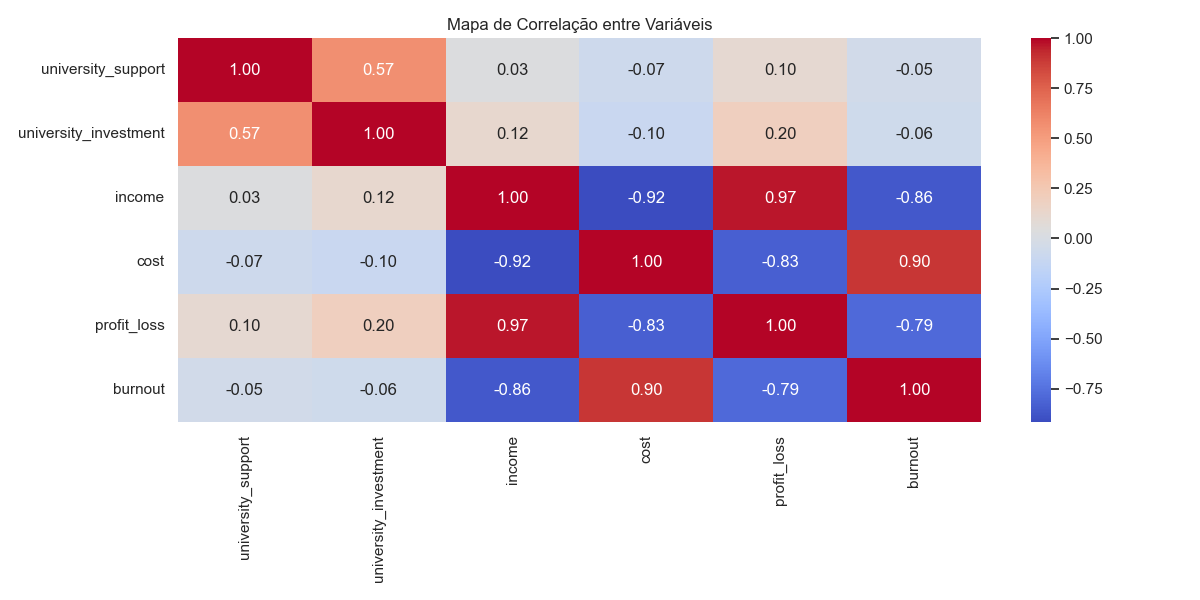
\includegraphics[width=1\textwidth]{imagens/heatmap_correlacao.png}
    \caption{Correlação das variáveis coletadas na simulação do modelo}
    \label{fig:correlacao-heatmap}
\end{figure}

\subsection{Interdependência entre Custo e Ganho do Conselheiro}

Conforme ilustrado na Figura~\ref{fig:dispersao-custo-ganho}, observa-se que conselheiros com níveis remuneratórios mais elevados tendem a apresentar custos associados proporcionalmente inferiores. 
Essa relação corrobora os achados de diversos estudos na literatura \cite{Judge2010, Jung2015, Chao2015, OrtinAngel2004, Singh2010}, os quais indicam que remunerações mais atrativas estão vinculadas a uma série de benefícios organizacionais, como a diminuição das taxas de rotatividade, a redução de custos operacionais indiretos, bem como o aumento da produtividade e da satisfação dos profissionais. Tais evidências sugerem que estruturas salariais mais competitivas podem estar associadas a menores custos secundários para a organização.

\begin{figure}[H]
    \centering
    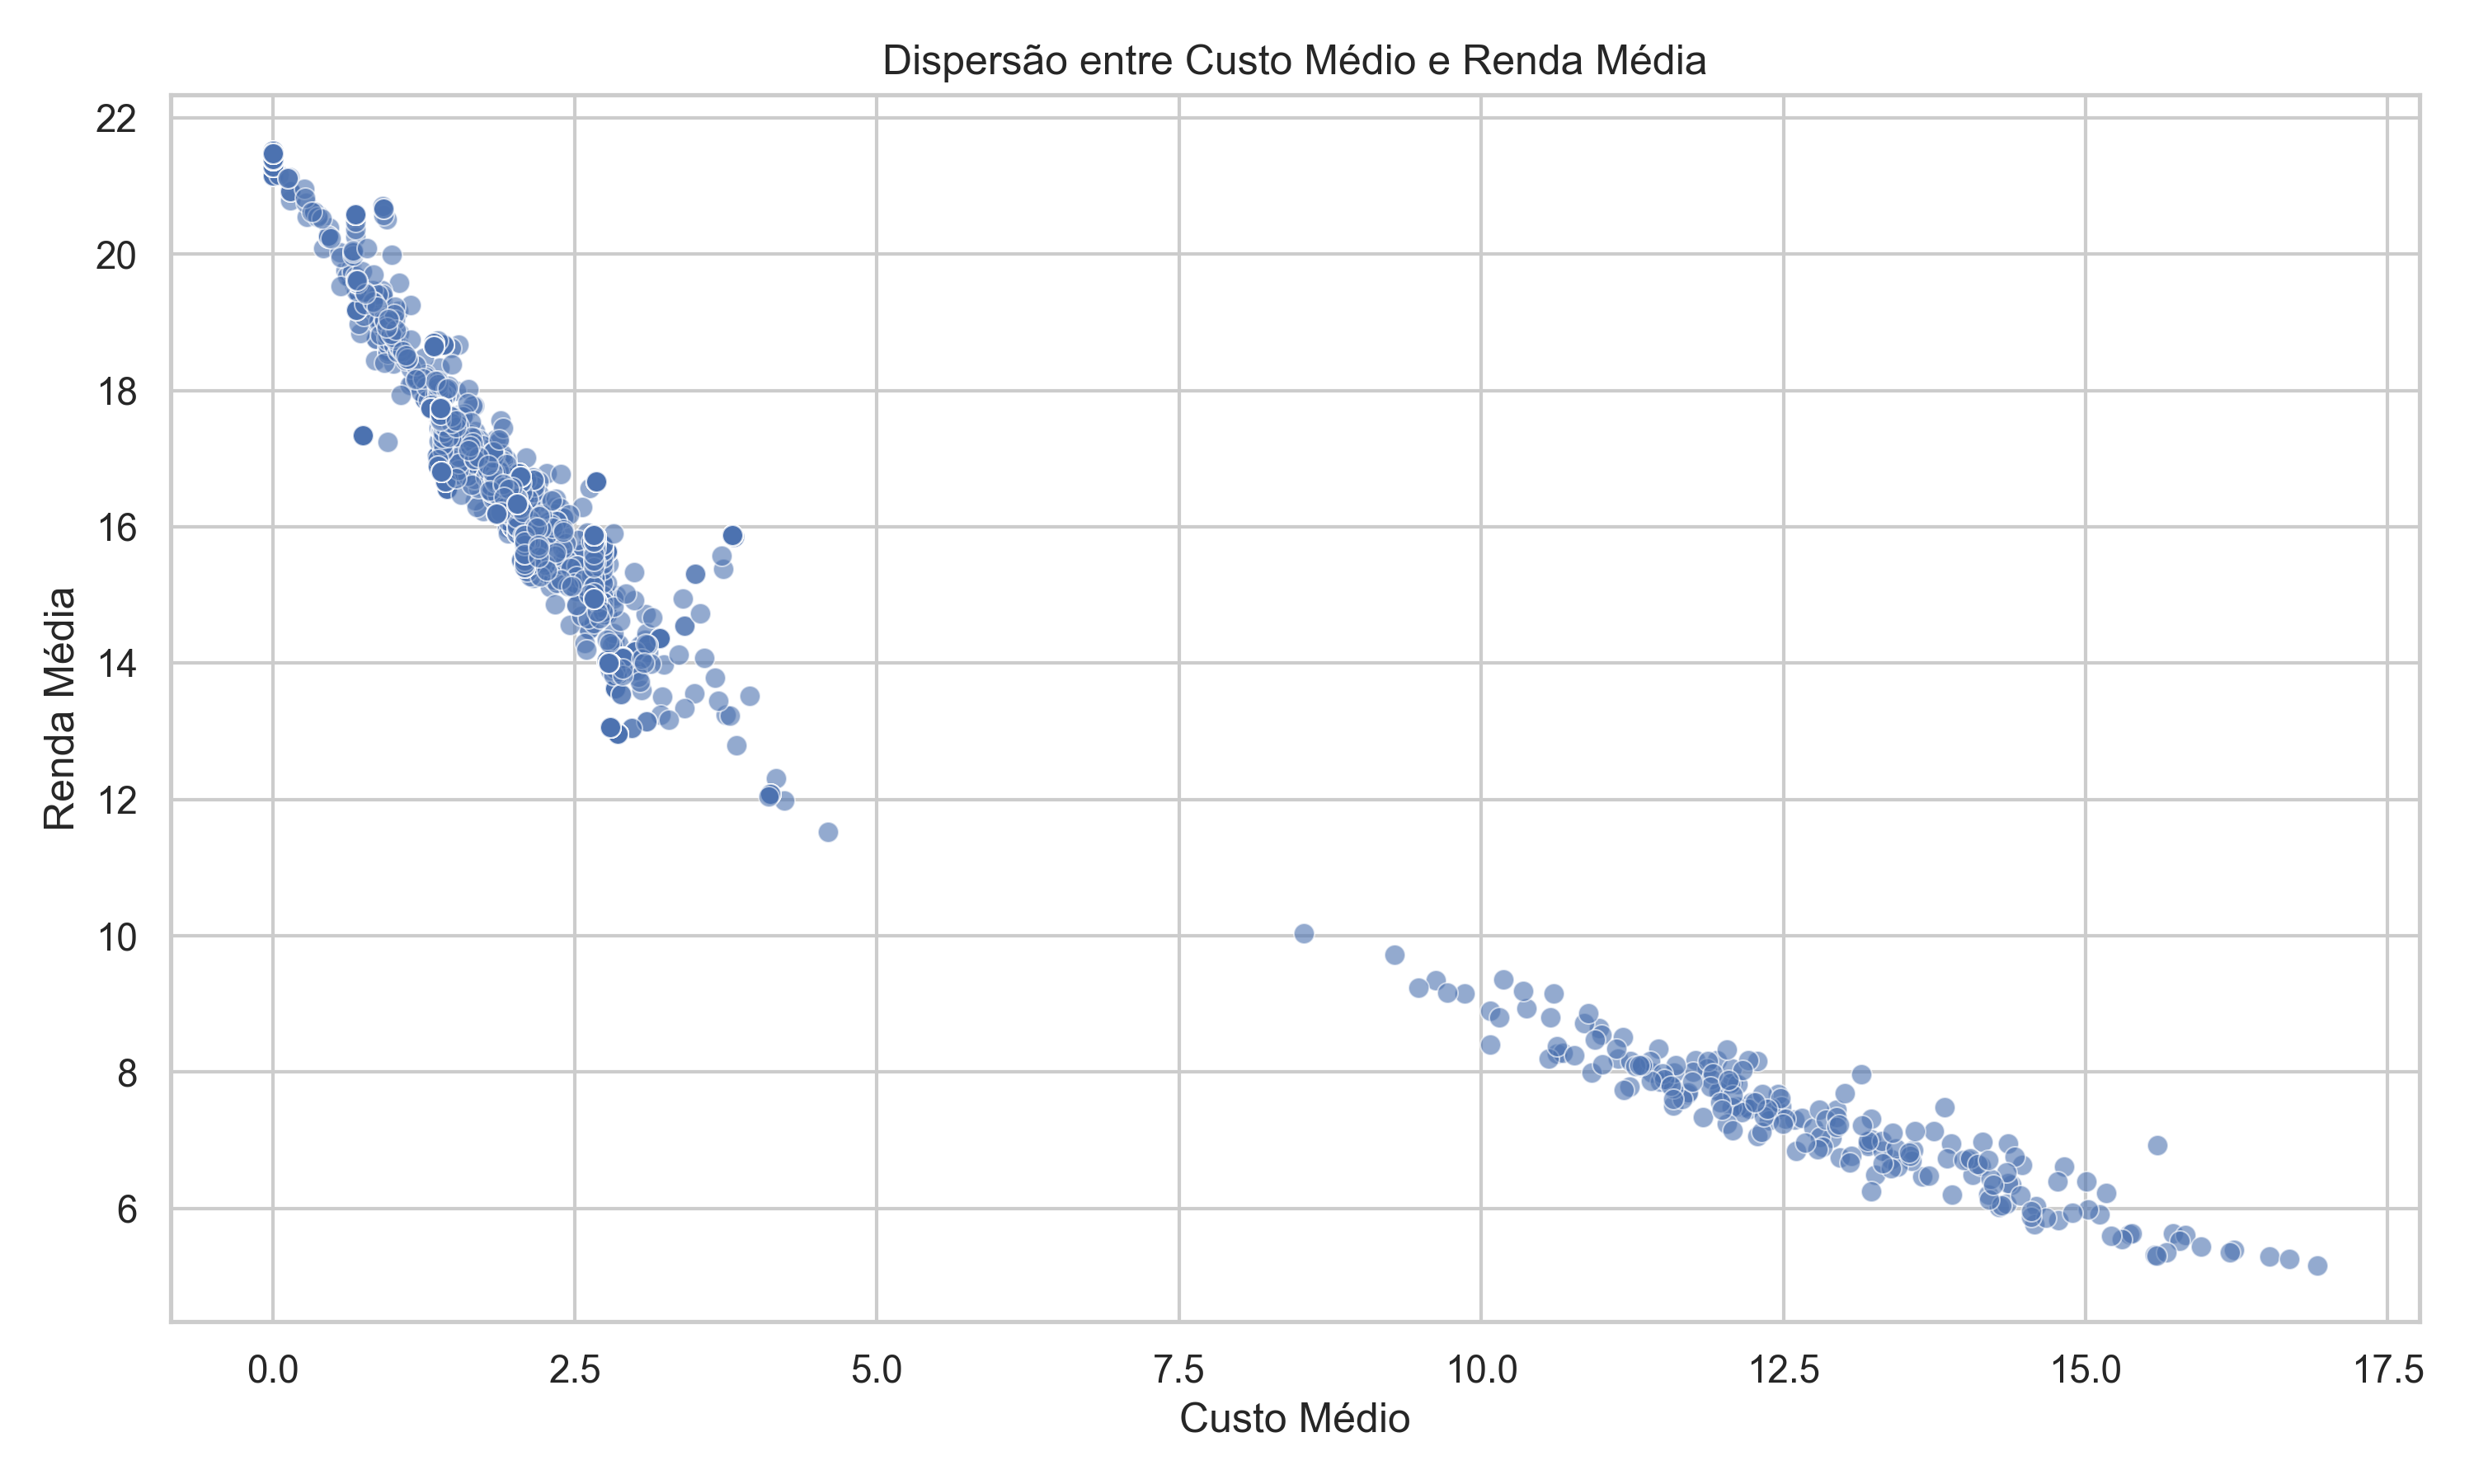
\includegraphics[width=1\textwidth]{imagens/dispersao-custo-ganho.png}
    \caption{Dispersão das variáveis Custo Médio x Renda Média}
    \label{fig:dispersao-custo-ganho}
\end{figure}

\subsection{Interdependência entre Custo e Ganho do Conselheiro e Correlação com a incidência de Burnout}

\begin{sloppypar}    
Conforme ilustrado na Figura~\ref{fig:dispersao-custo-lucro-burnout}, observa-se que o aumento dos custos profissionais e a redução dos lucros médios do conselheiro estão diretamente associados ao crescimento da incidência de burnout. 
Esse fenômeno é amplamente discutido na literatura. Segundo \citeonline{hardarson2021emotional}, o burnout entre professores está relacionado a múltiplos fatores, como a falta de reconhecimento, o excesso de burocracia, as dificuldades nas interações com a gestão, a perda de autonomia, a sobrecarga de trabalho e a desvalorização das políticas educacionais.

Nesse contexto, o modelo adotado neste artigo — baseado na proposta de \citeonline{Zhang2020Burnout} — avalia os custos e ganhos do conselheiro a partir de variáveis objetivas e subjetivas, considerando diferentes horizontes temporais (curto, médio e longo prazo). À medida que os custos se acumulam, crescem também as incertezas quanto ao futuro profissional, intensificando o estresse e favorecendo a consolidação de um ciclo persistente de burnout.
\end{sloppypar}

\begin{figure}[H]
    \centering
    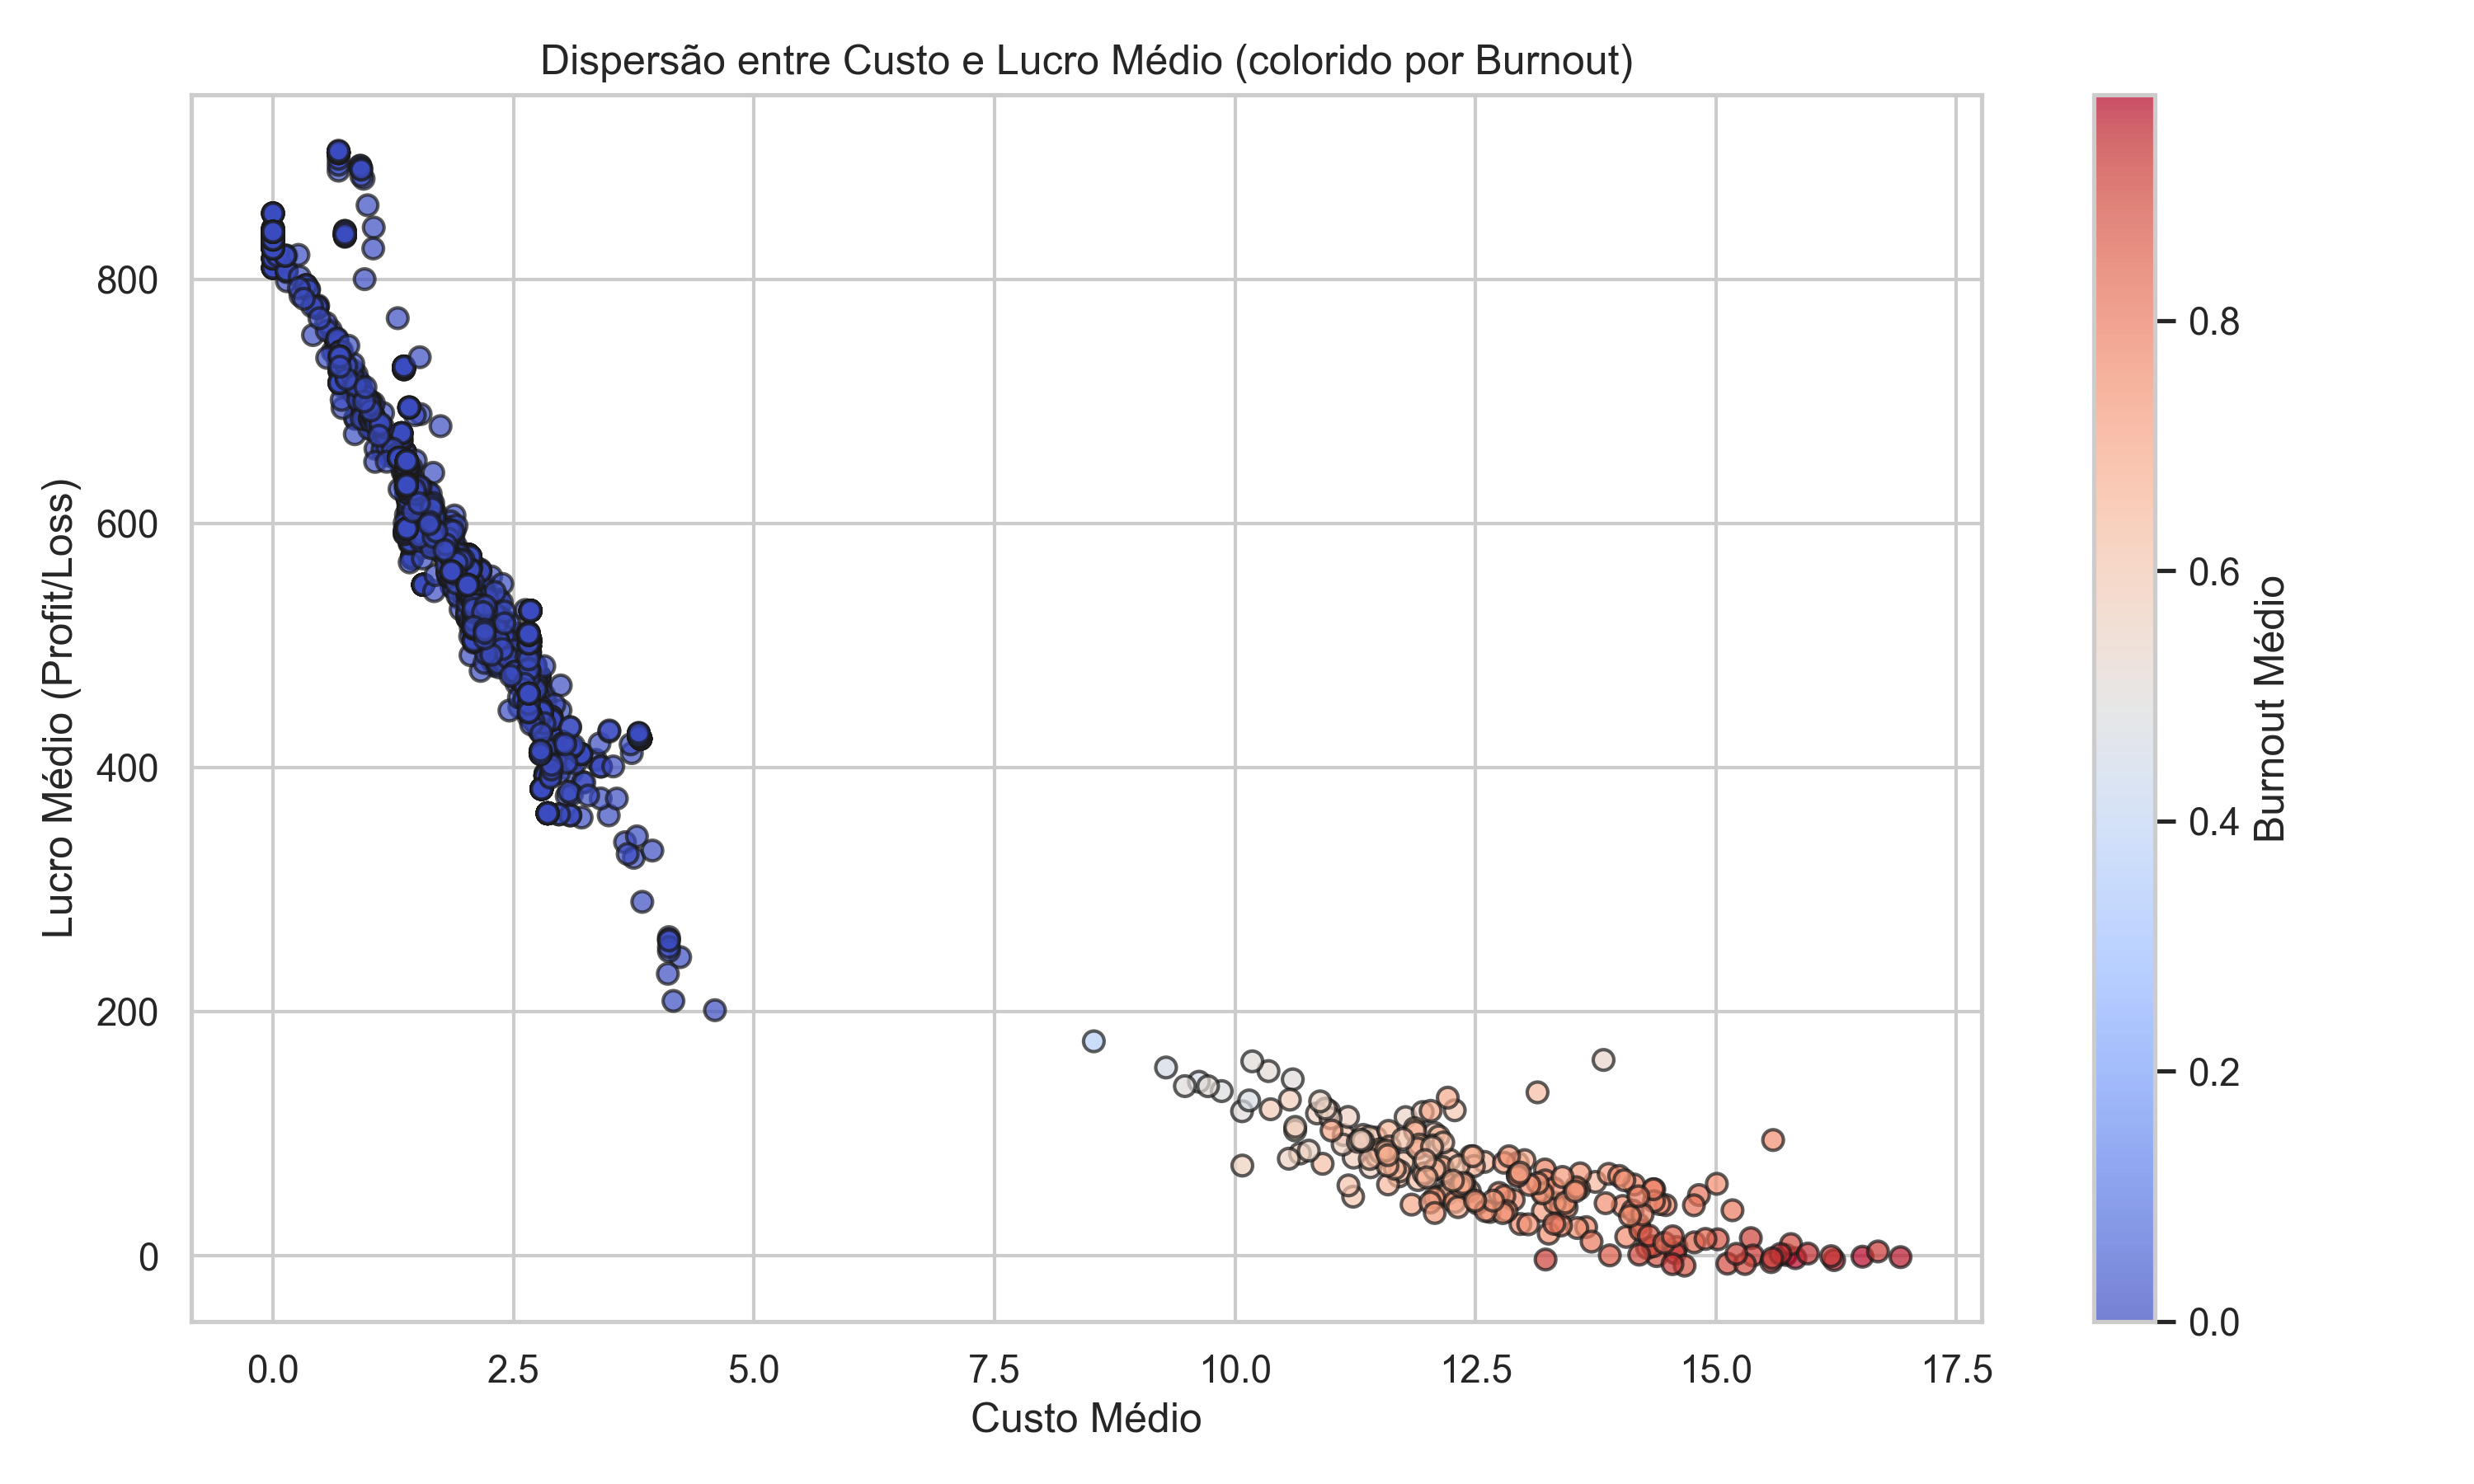
\includegraphics[width=1\textwidth]{imagens/dispersao-custo-lucro-colorido-por-burnout.png}
    \caption{Dispersão das variáveis Custo Médio x Lucro Médio - por Burnout}
    \label{fig:dispersao-custo-lucro-burnout}
\end{figure}

\subsection{Restrições da Simulação}
O modelo proposto apresenta diversas limitações, sendo as principais descritas a seguir:

\begin{itemize}
    \item Conforme o modelo proposto por \citeonline{Zhang2020Burnout}, os conselheiros são considerados agentes racionais que tomam decisões desprovidas de emoções. No entanto, essa suposição impede o modelo de capturar como os ciclos de burnout aumentam os custos e levam os conselheiros a adotarem estratégias ineficazes, influenciadas pelo desgaste emocional.

    \item A universidade é tratada como um agente externo com influência limitada sobre o tabuleiro. Contudo, em contextos organizacionais reais, a instituição exerce impacto direto e significativo nas estratégias adotadas pelos jogadores, o que não é adequadamente refletido no modelo.

    \item O problema das \( N \) Rainhas pode não ser a representação mais adequada para ilustrar dinâmicas organizacionais reais, devido à sua simplicidade, ao número restrito de iterações e à ausência de um componente temporal dinâmico \cite{rozier, BarrRao2006}.
\end{itemize}



\section{Conclusões}
Os resultados apresentados neste estudo baseiam-se em análises de correlação entre variáveis, como a forte relação negativa entre burnout e ganho financeiro (\( r = -0{,}86 \)) e a relação positiva com o aumento de custos (\( r = 0{,}90 \)). No entanto, é importante destacar que correlação não implica necessariamente causalidade, especialmente em cenários dinâmicos e complexos, dadas as limitações tanto do modelo-base \cite{Zhang2020Burnout} quanto do modelo proposto neste trabalho. Para fortalecer a evidência dessas relações, seriam necessários estudos com maior abrangência temporal ou realizados em ambientes controlados que possibilitem o isolamento de variáveis.

Outra limitação relevante diz respeito ao escopo do modelo original \cite{Zhang2020Burnout}, desenvolvido especificamente para conselheiros em instituições universitárias — um contexto particular que pode não refletir as dinâmicas presentes em outros setores corporativos. Assim, a generalização dos resultados para diferentes contextos organizacionais deve ser feita com cautela e requer investigação adicional.

Para superar essas limitações, este estudo poderia incorporar abordagens mistas, combinando métodos quantitativos com entrevistas qualitativas, de modo a explorar fatores subjacentes às correlações observadas. Além disso, seria valioso expandir ou replicar o modelo em diferentes organizações e setores, buscando maior robustez e generalização dos resultados. Estudos anteriores, como os de \citeonline{maslach2001burnout} e \citeonline{Slusarz2022}, já enfatizaram a importância de considerar múltiplos fatores ao interpretar dados relacionados ao burnout.

Dessa forma, conclui-se que, embora o trabalho proposto tenha atingido seu objetivo principal — identificar correlações entre ganhos financeiros, custos e incidência de burnout —, há espaço significativo para aprofundamento e aprimoramento da análise.



\newpage
\begin{apendices}

\chapter{Tabela Referência - Algoritmo Genético}


\end{apendices}

\newpage
\bibliographystyle{abntex2-alf}
\bibliography{referencias}

\end{document}
